\documentclass[12pt,xcolor=table]{beamer}
\usepackage[utf8]{inputenc}
\usepackage{listings}
\usepackage{color}

\usecolortheme{rose}
\definecolor{color}{HTML}{009900}
\usetheme{Darmstadt}
\setbeamertemplate{navigation symbols}{}
%\setbeamercolor{frametitle}{fg=white}
\setbeamercolor{structure}{bg=black, fg=color}

\setbeamertemplate{section in toc}{%
  {\color{orange!70!black}\inserttocsectionnumber.}~\textbf{\inserttocsection}}
\setbeamercolor{section in toc}{fg=black}
\setbeamercolor{subsection in toc}{bg=white,fg=black}
\setbeamercolor{bibliography item}{fg=black}
\setbeamercolor*{bibliography entry author}{fg=black}
\setbeamertemplate{subsection in toc}{%
  \hspace{1.2em}{\color{orange}\rule[0.3ex]{3pt}{3pt}}~\inserttocsubsection\par}


\title{Verifica automatica della proprietà di\\ sicurezza forte}

\author{Gianluca Lutero}
\institute{Alma Mater Studiorum Bologna\\Crittografia}
\date{}

\begin{document}

\begin{frame}{}
    \maketitle
\end{frame}

\begin{frame}{Outline}
    \begin{itemize}
        \item Introduzione
        \item Calcolo dei processi
        \item Segretezza forte
        \item Implementazione
        \item Algoritmo di risoluzione
    \end{itemize}
\end{frame}

\begin{frame}{Introduzione}
    
\end{frame}

\section{Calcolo dei processi}
\subsection{}
\begin{frame}{Calcolo dei processi}
    \begin{figure}[h]
        \centering
        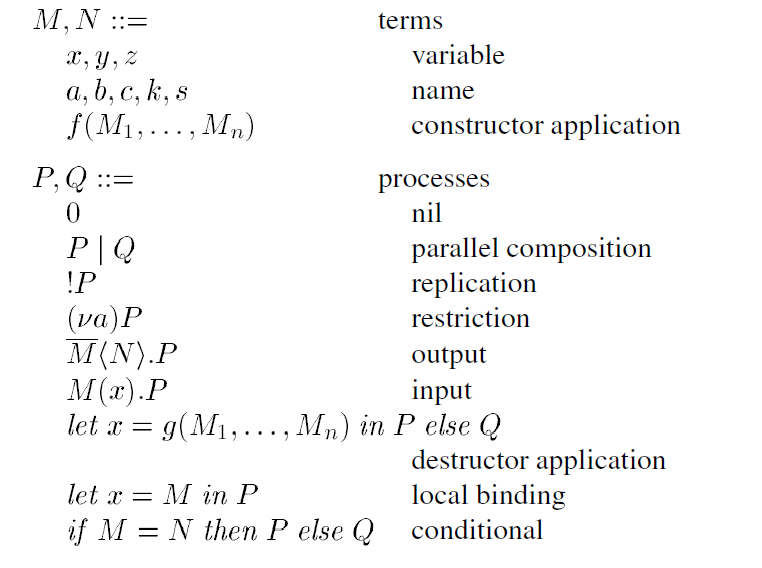
\includegraphics[scale=0.5]{Relazione/Immagini/calcolo.PNG}
    \end{figure}
\end{frame}

\section{Segretezza forte}
\subsection{}
\begin{frame}{Segretezza forte}
    \begin{block}{Segretezza}
        L'avversario non può ottenere il valore del segreto.
    \end{block}
    \vspace{5mm}
    \begin{block}{Segretezza forte}
        Questa proprietà esprime l'impossibilità da parte dell'avversario di sapere quando il valore del segreto cambia.
    \end{block}
\end{frame}

\begin{frame}{Equivalenza osservazionale}
    Si definisce equivalenza osservazionale $\approx$ la piú grande relazione simmetrica $R$ tra processi chiusi tale che $PRQ$ implica:\\
    \begin{enumerate}
        \item se $P \Downarrow m$ allora $Q \Downarrow m$
        \item se $P \rightarrow P'$ allora esiste $Q'$ tale che $Q \rightarrow^* Q'$ e $P'RQ'$
        \item $C[P]RC[Q]$ per tutti i contesti di valutazione chiusi $C$.
    \end{enumerate}
\end{frame}

\begin{frame}{}
    \begin{block}{}
        Viene utilizzata la definizione di equivalenza osservazionale per esprimere la proprietà di segretezza forte nel calcolo dei processi.
    \end{block}
    
    \begin{block}{Proprietà}
        Il processo $P_0$ preserva la segretezza forte delle sue variabili libere se e solo se per ogni sostituzione chiusa $\sigma$ e $\sigma'$ di dominio $fv(P_0)$ , $\sigma P_0 \approx \sigma' P_0$.
    \end{block}
\end{frame}


\section{Implementazione}
\begin{frame}{Implementazione}

\end{frame}

\section{Algoritmo di risoluzione}
\begin{frame}{Algoritmo di risoluzione}
    
\end{frame}

\end{document}